\documentclass{beamer}

\usepackage[utf8]{inputenc}
%\usepackage[T1]{fontenc}
%\usepackage[latin1]{inputenc}

\usetheme{Warsaw}

\title[Signal segmentation]{Functionnal data analysis applied to neurology}
\author{Clément Bonvoisin, Pierre Ludmann}
\institute{CMLA (ENS Cachan), Cognac-G (Paris V)}
\date{09/04/2014}

\graphicspath{neuro-seg/}
\setbeamersize{text margin left=1.4cm}
\begin{document}
\setbeamertemplate{navigation symbols}{}
\setbeamertemplate{footline}[frame number]
%\addtobeamertemplate{footline}{\hfill\insertframenumber/\inserttotalframenumber}

\begin{frame}
\titlepage
\end{frame}

\begin{frame}
\frametitle{Plan}
  \tableofcontents[hideallsubsections]
\end{frame}

\AtBeginSection[]
{
  \begin{frame}
  \tableofcontents[currentsection, hideothersubsections]
  \end{frame} 
}

\section{Familiarisation avec le problème}
\subsection{Protocole expérimental}

\begin{frame}
\frametitle{}

\begin{itemize}

\item[Trajet] du patient : 
\item environ 6 secondes à l'arrêt
\item marche sur 10 mètres
\item demi-tour
\item marche sur 10 mètres

\item[Capture] des signaux par deux centrales inertielles : 
\item fixées à la ceinture et au pied droit
\item accélérations et vitesses angulaires
\item enregistrées à 20 Hz
\item replacées dans le référentiel\\(antéro-postérieure, medio-latérale, verticale)

\end{itemize}

\end{frame}

\subsection{Visualisation des données}
\begin{frame}

\begin{itemize}

\item[Fichiers] sous extension .txt ou .csv
\item Besoin de procédures pour importer au format .mat

\item[Fonction] d'affichage
\item Les différentes phases sont visibles sans besoin de modification

\item[$\Longrightarrow$] La segmentation automatique doit être rapide et précise, au moins autant que l'œil

\end{itemize}

\end{frame}

\begin{frame}
\frametitle{Exemple d'aquisition d'un capteur fixé à la ceinture}
\hspace*{-2.8cm}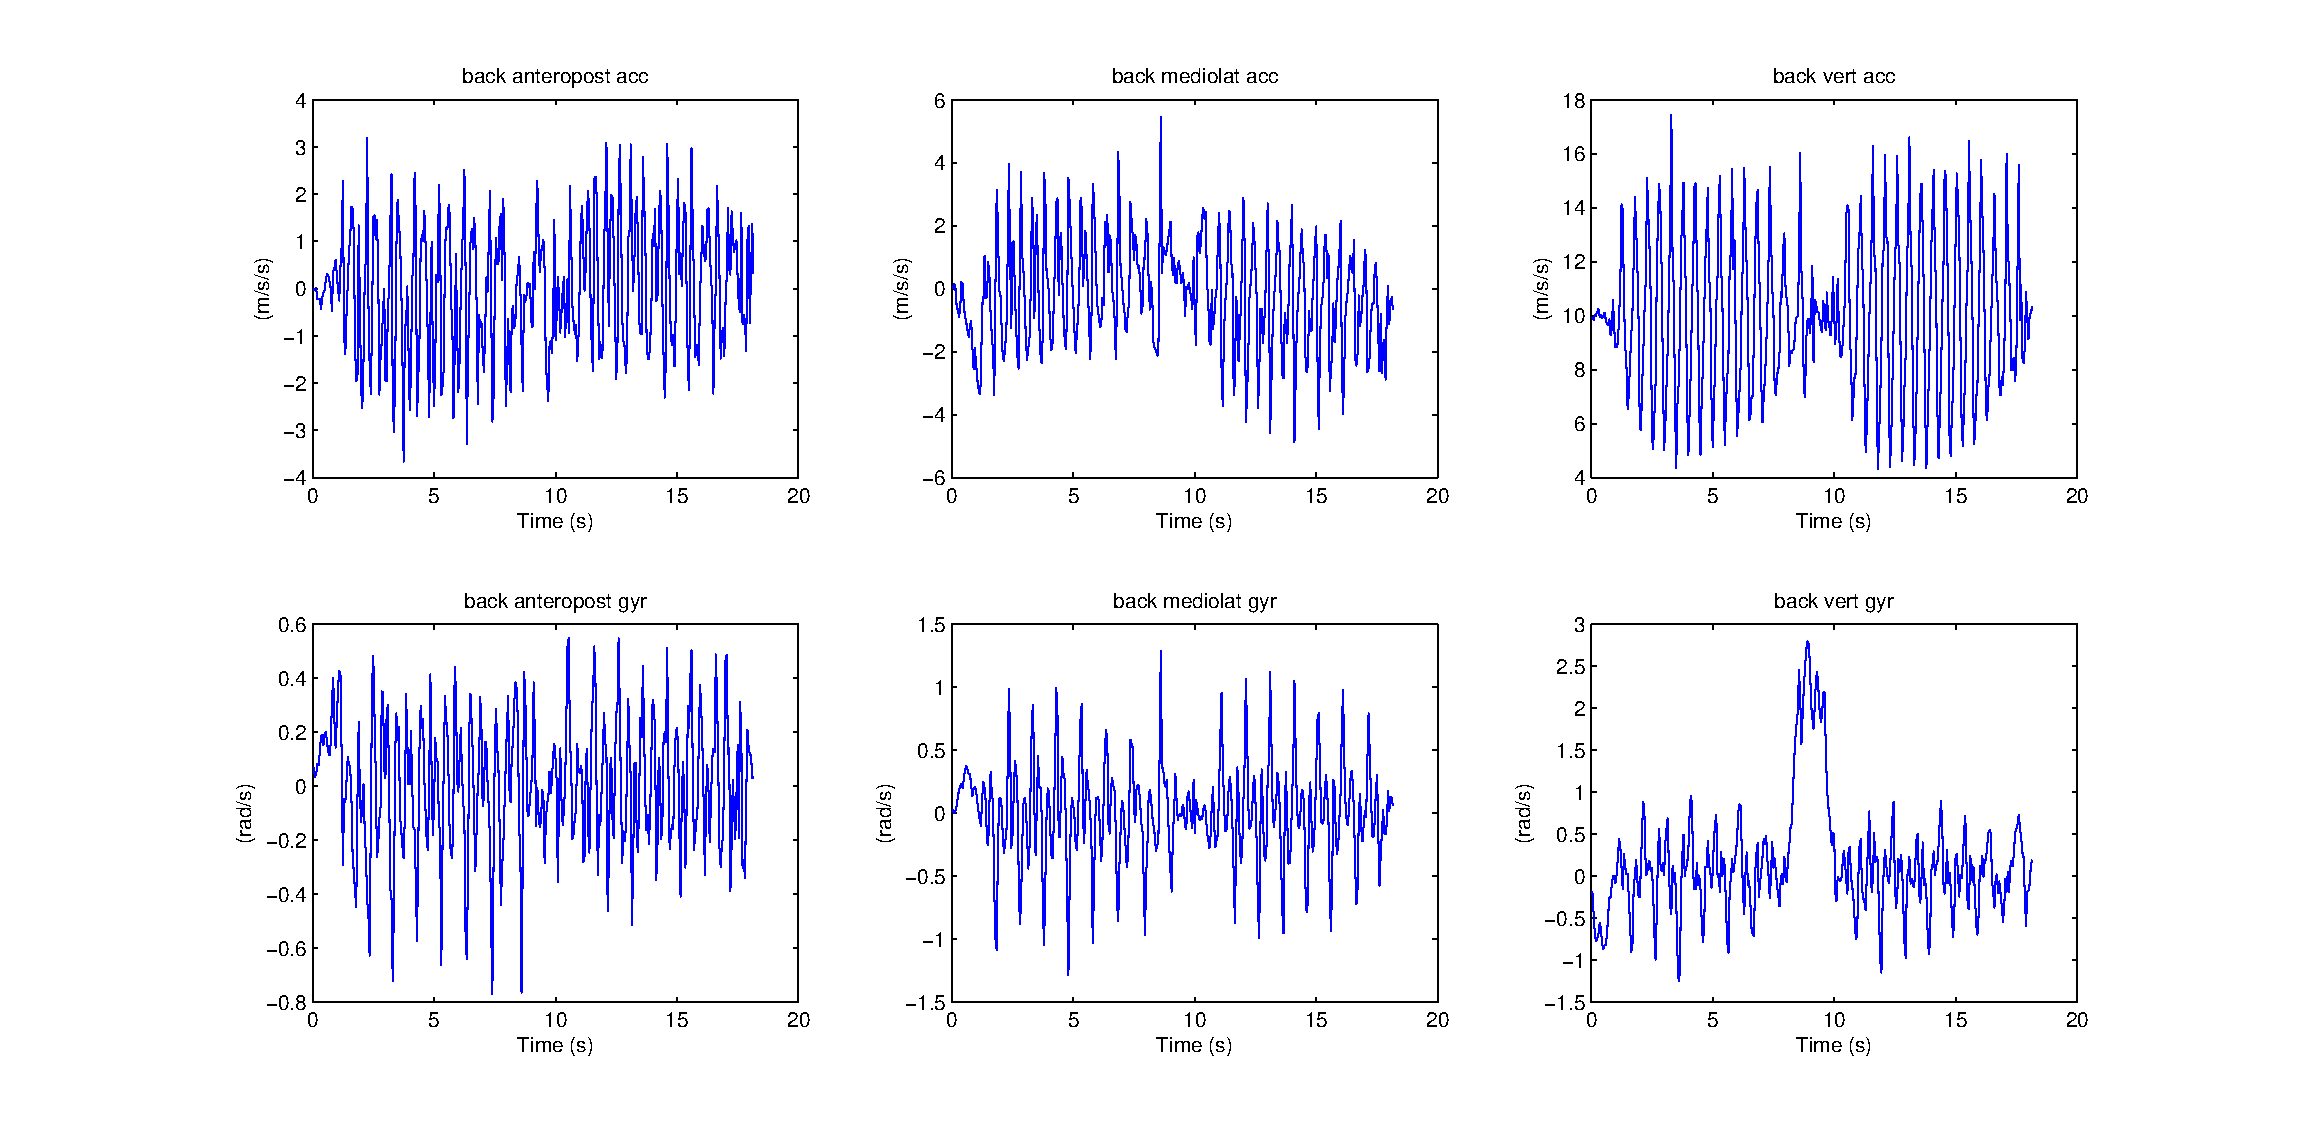
\includegraphics[scale=0.4]{examplevisuback}

\end{frame}

\begin{frame}
\frametitle{Exemple d'aquisition d'un capteur fixé au pied}
\hspace*{-2.8cm}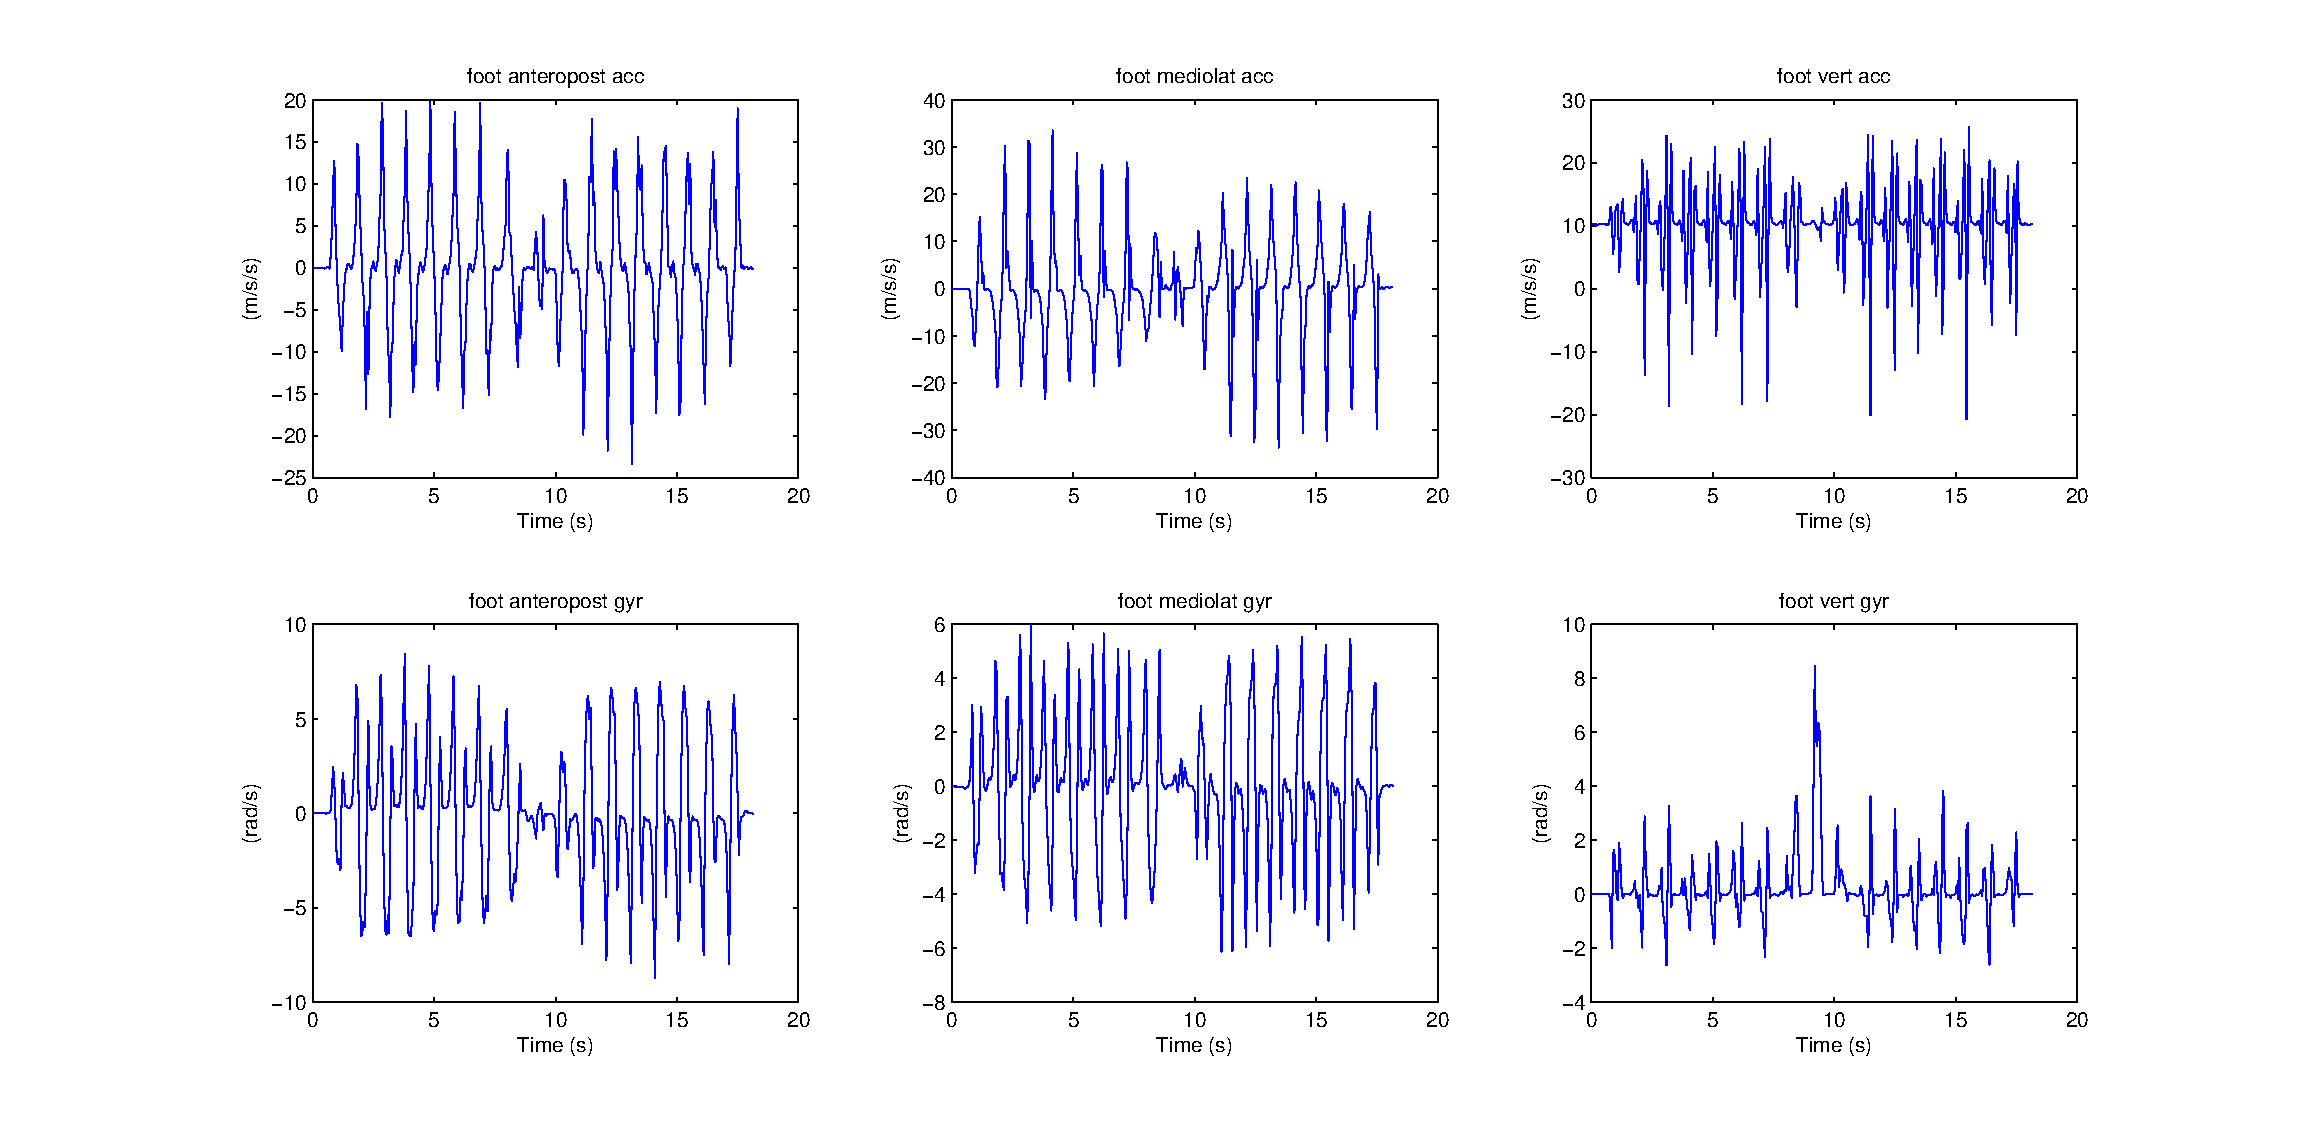
\includegraphics[scale=0.4]{examplevisufoot}

\end{frame}

\section{Approche par fenêtres}
\subsection{Avec Fourier}

\begin{frame}
\begin{itemize}
\item[Biblio] \emph{Classification of periodic activities using the Wasserstein distance}, L. Oudre, J. Jakubowicz, P. Bianchi, C. Simon

\item[Spectre] des fréquences de 0.5 à 5 Hz d'une fenêtre du signal

\item[Distance] de Wasserstein moins sensible aux décalages, utilisé dans le traitement de l'image et du son
\[d_W(g,h)=\int_0^\pi\left|\int_0^xg(t)-h(t)dt\right|dx\]

\item[Distance] point à point
\[d(x,y)=d_W(\frac x{||x||_1},\frac y{||y||_1})+\mu\cdot\left|\phantom{\frac{}{}}||x||_1-||y||_1\right|\]
\end{itemize}
\end{frame}

\begin{frame}
\frametitle{Application sur les vitesses angulaires à la ceinture :\\fenêtres de 16 et 32 échantillons, recouvrement de 75\%}
\hspace*{-1.8cm}\includegraphics[scale=0.47]{examplewasser16gyr}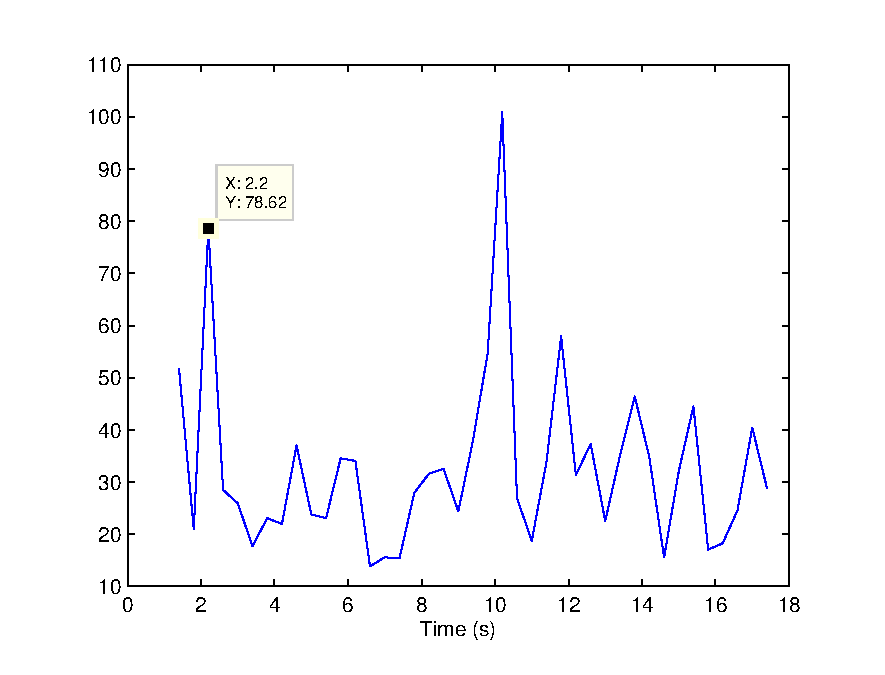
\includegraphics[scale=0.47]{examplewasser32gyr}
\end{frame}

\subsection{Avec des statistiques}
\begin{frame}
\begin{itemize}
\item[Beaucoup] d'extracteurs proposés dans la littérature :
\item moyennes de $a_{ML}+a_V$, $a_{AP}$ et $a_V$ ;
\item écarts-type de $a_{AP}+a_V$ et $a_{ML}$ ;
\item médiane de $a_V$ ;
\item 95-quantile de $a_{ML}$ ; \emph{etc}

\item[Bons] résultats avec le kurtosis
\item[Taille] des fenêtres problématiques : compromis précision/lissage, difficile à moins de 100 Hz
\end{itemize}
\end{frame}

\begin{frame}
\hspace*{-2cm}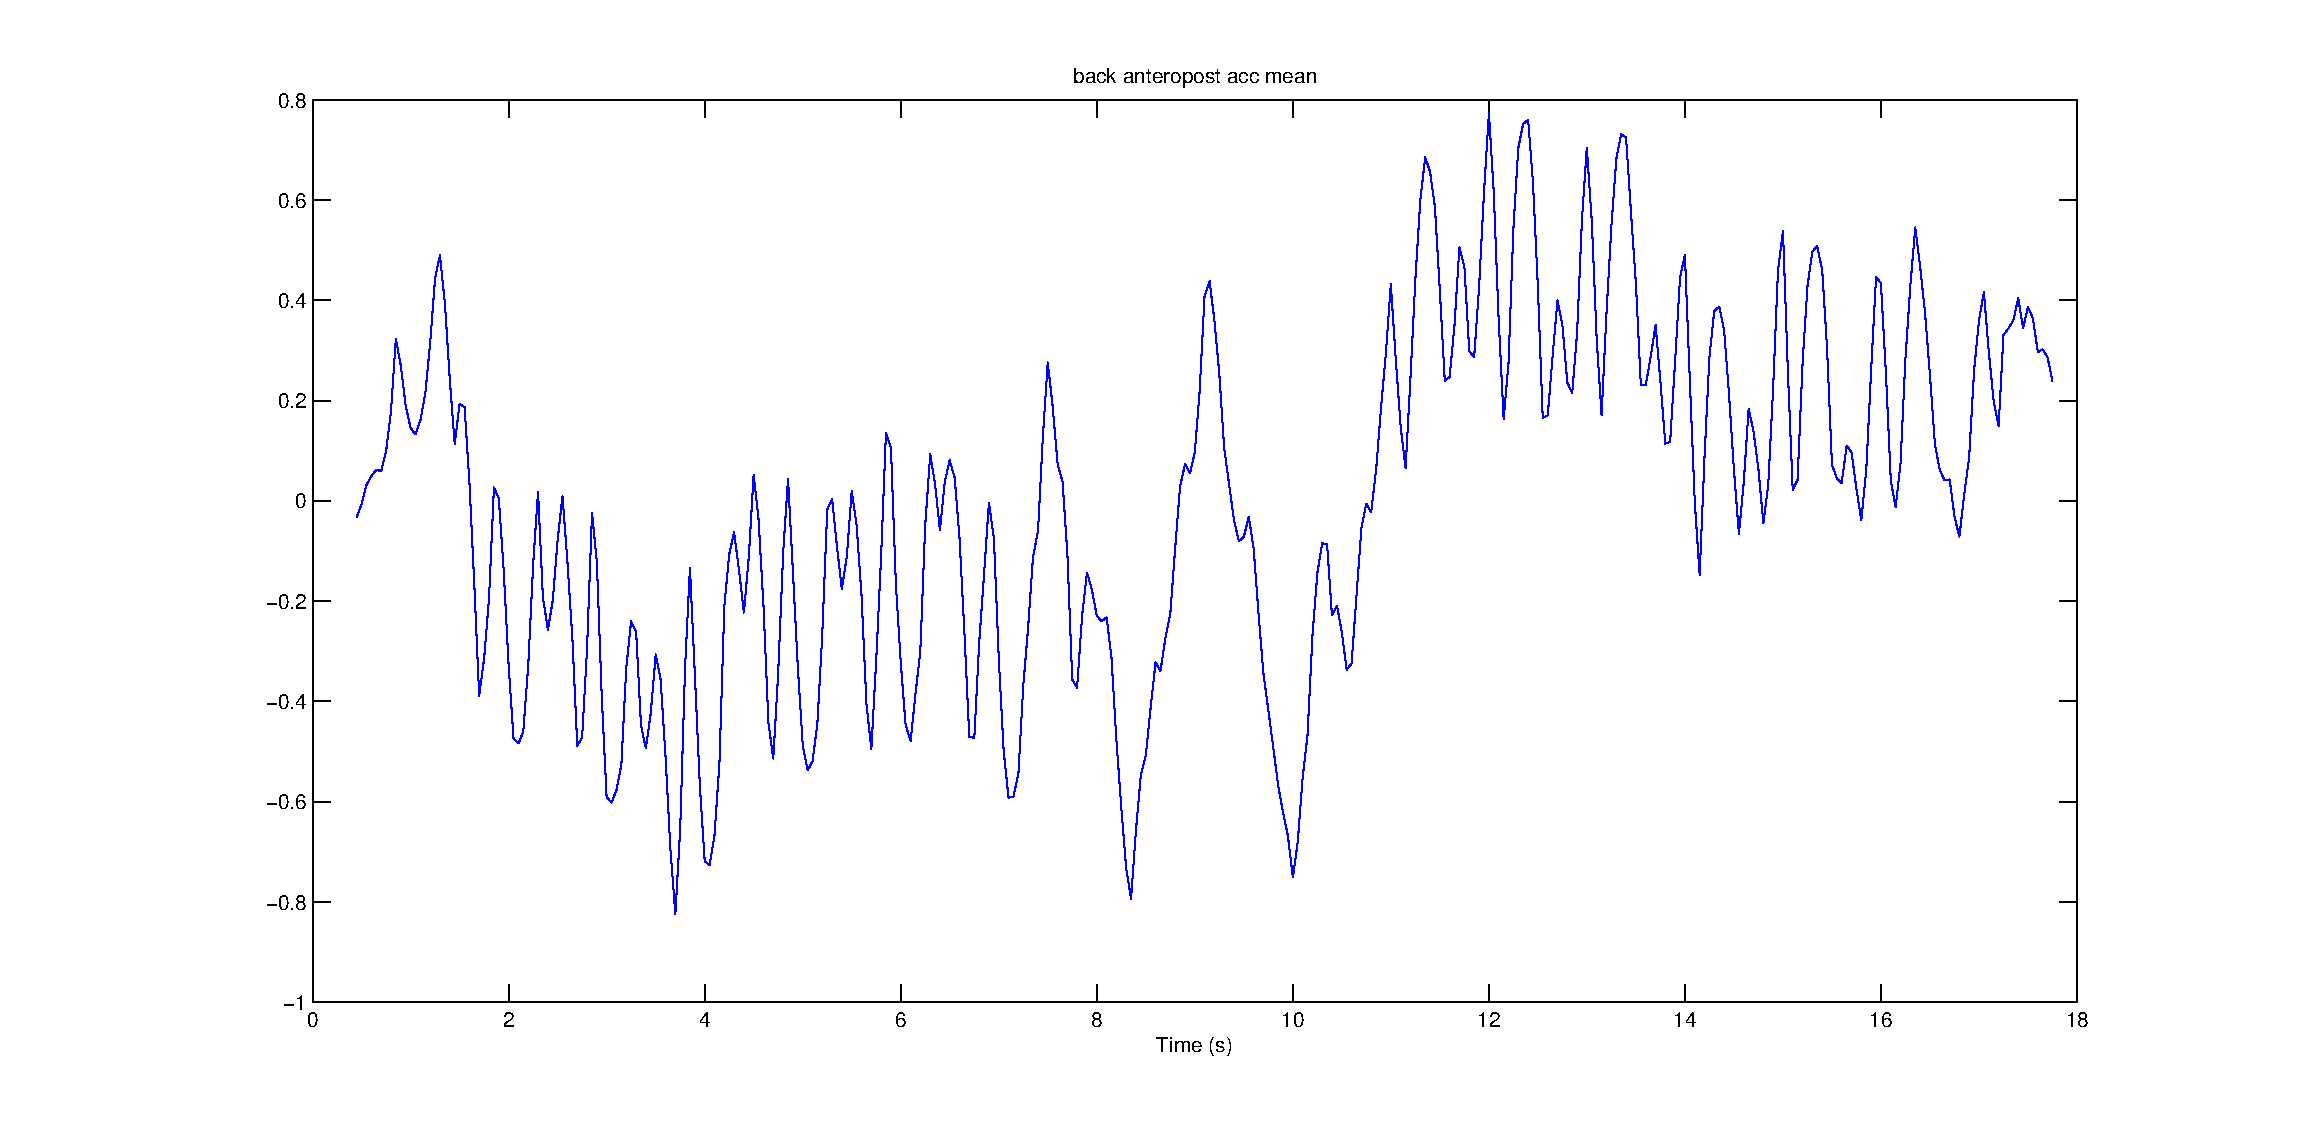
\includegraphics[height=4.4cm,width=6.9cm]{examplew16moyAap}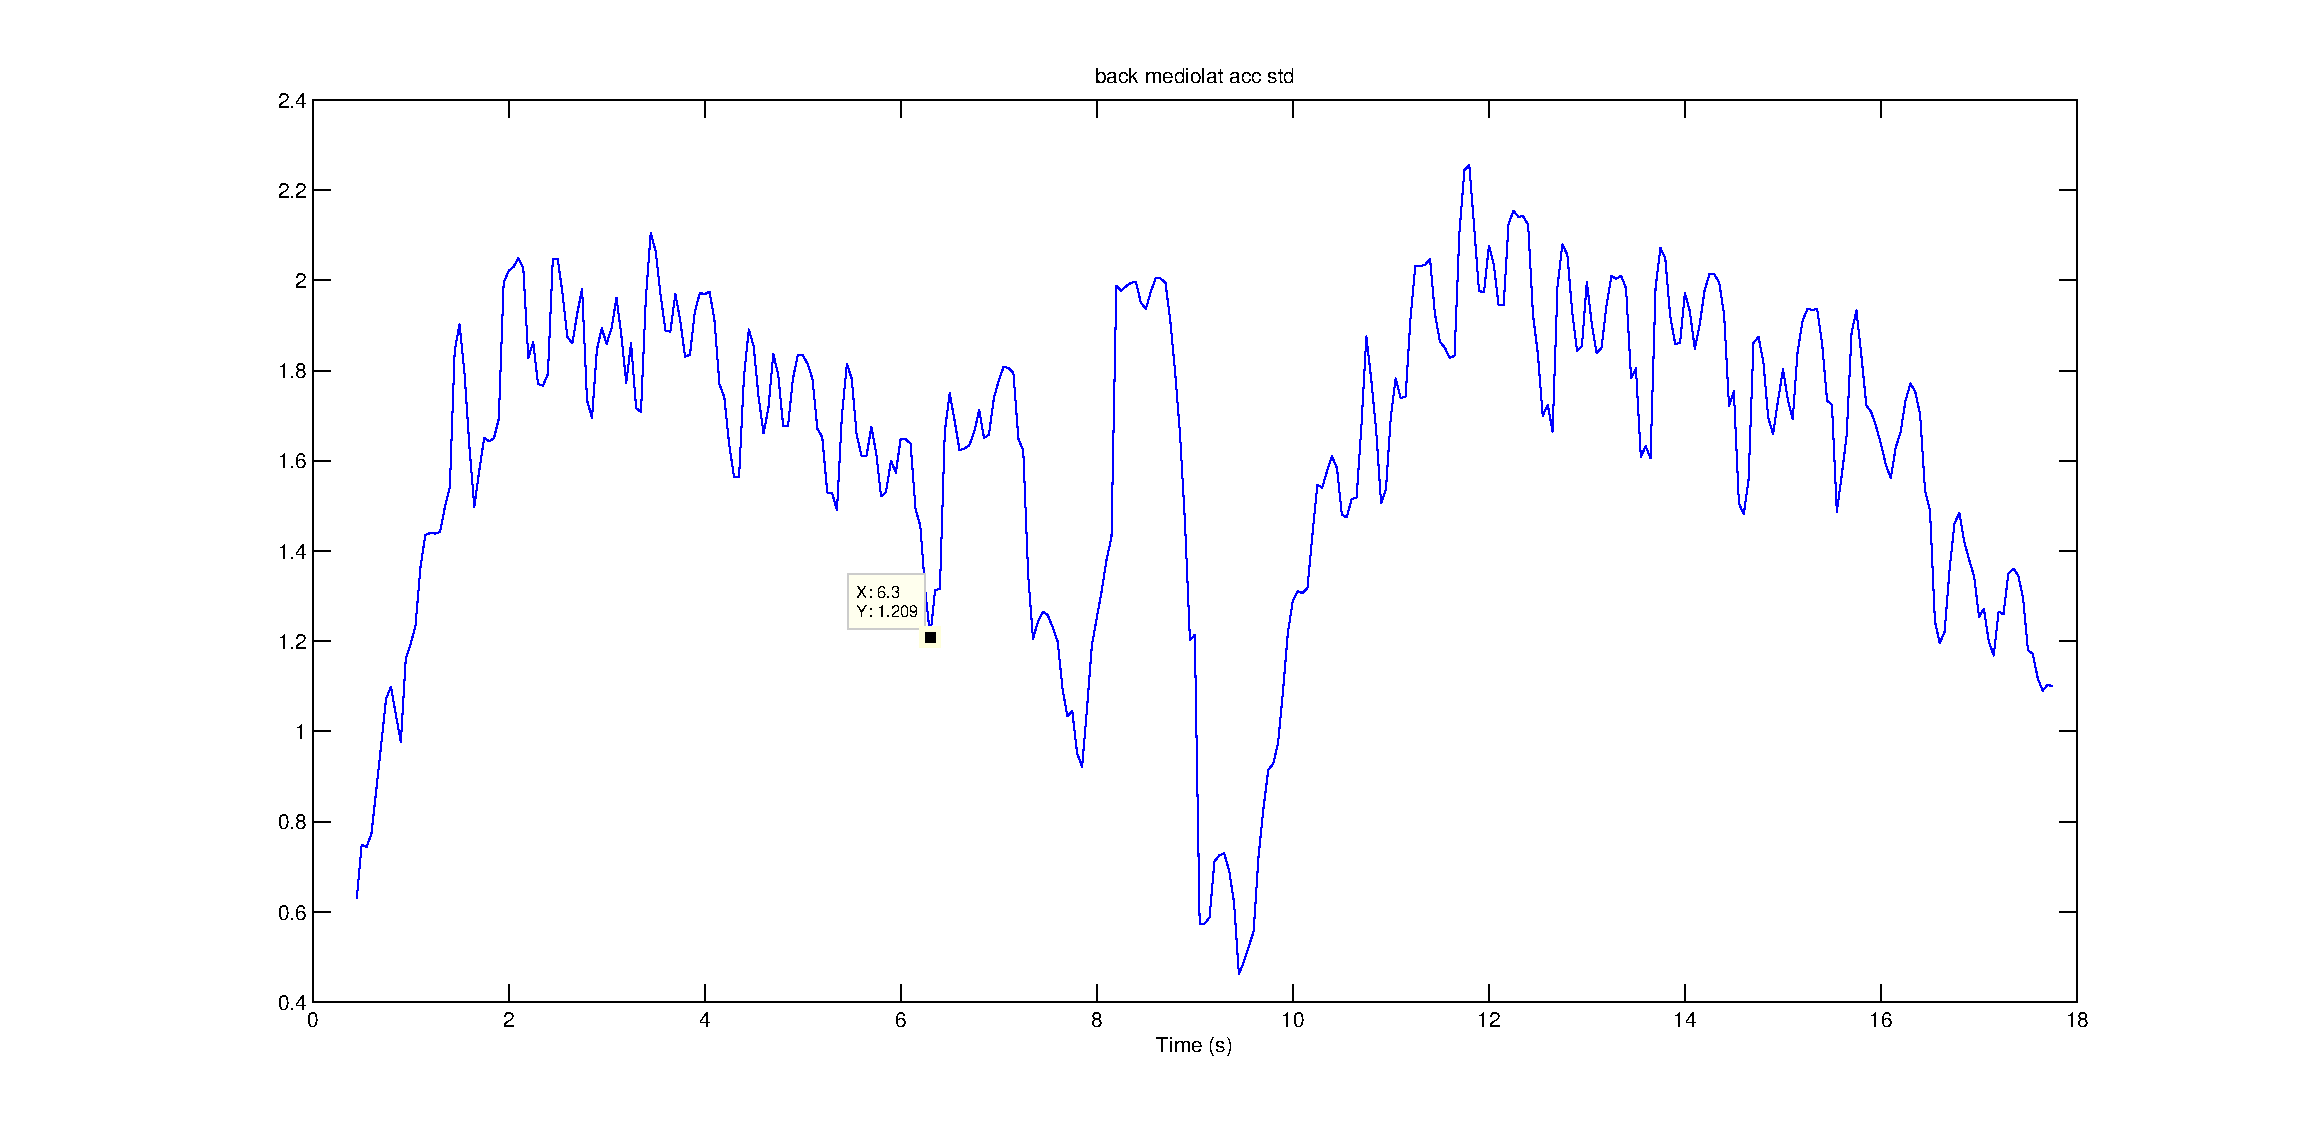
\includegraphics[height=4.4cm,width=6.9cm]{examplew16stdAml}
\\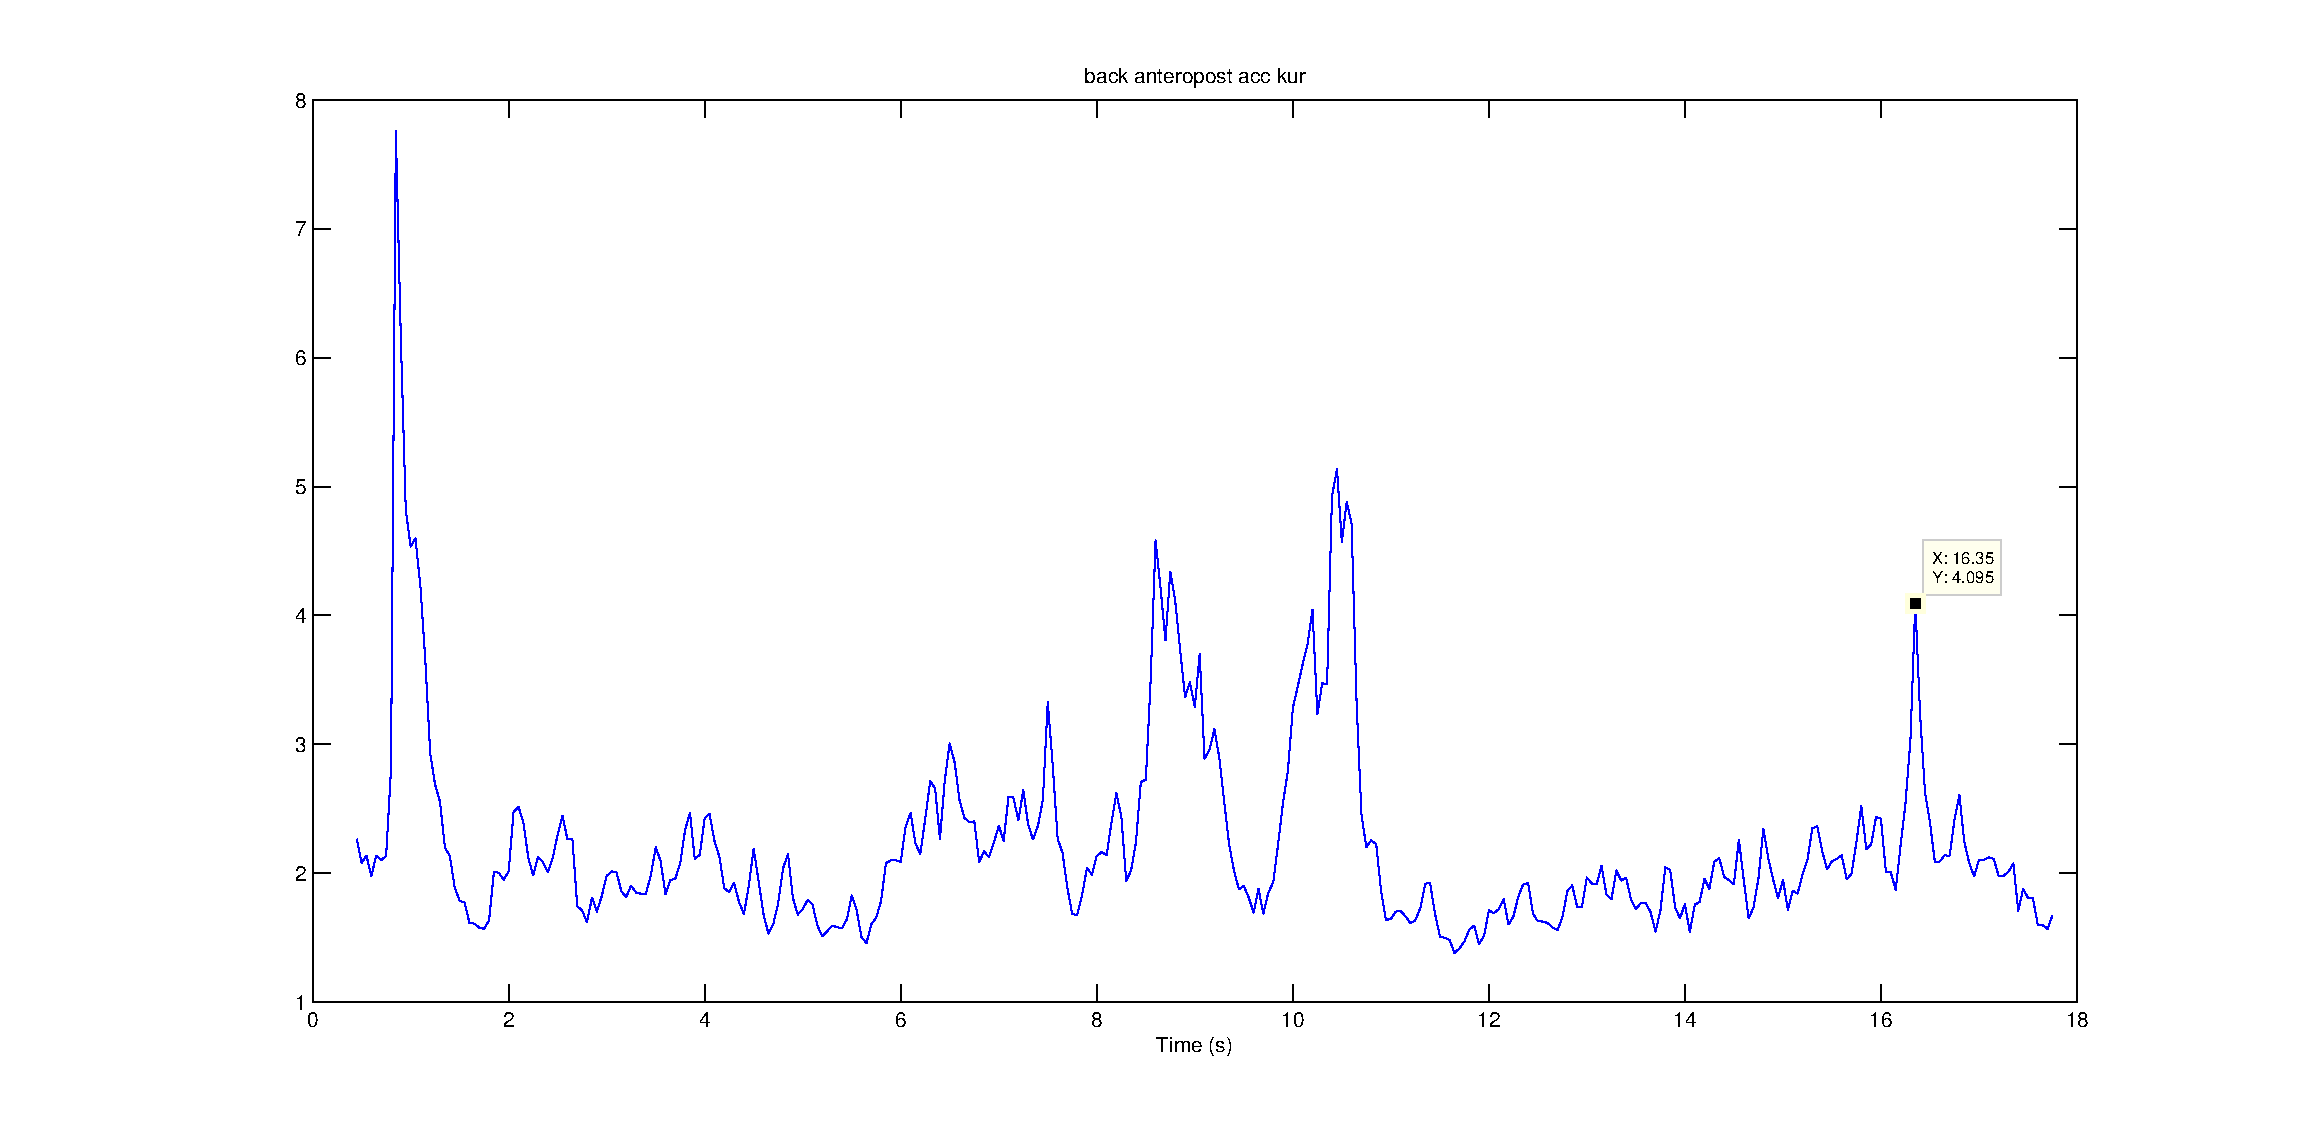
\includegraphics[height=4.4cm]{examplew16kurAap}
\end{frame}

\section{Algorithme CUSUM}
\subsection{Fonctionnement}

\begin{frame}
\begin{itemize}
\item[Biblio] \emph{Detection of Abrupt Changes : Theory and Application},\\
M. Basseville, I. V. Nikiforov (1993)
\item[Proposé] par E. S. Page en 1954
\item[Basé] sur des maxima de vraissemblance estimée
\[\tilde\varLambda_1^N(k)=\inf_{\tilde\theta_0}\sup_{\theta_0}\sup_{\theta_1}\ln\left[\frac{\prod_{i=1}^{k-1}p_{\theta_0}(y_i)\cdot\prod_{i=k}^Np_{\theta_0}(y_i)}{\prod_{i=1}^Np_{\tilde\theta_0}(y_i)}\right]\]
\[\hat t_0=\arg\max_{1\le k\le N}\tilde\varLambda_1^N(k)\]
\item[Hypothèse] de signaux indépendants sous loi normale
\item[Utilisé] sur la norme des accélérations et la rotation par dichotomie
\end{itemize}
\end{frame}

\subsection{Premiers résultats}

\begin{frame}
\hspace*{-2.8cm}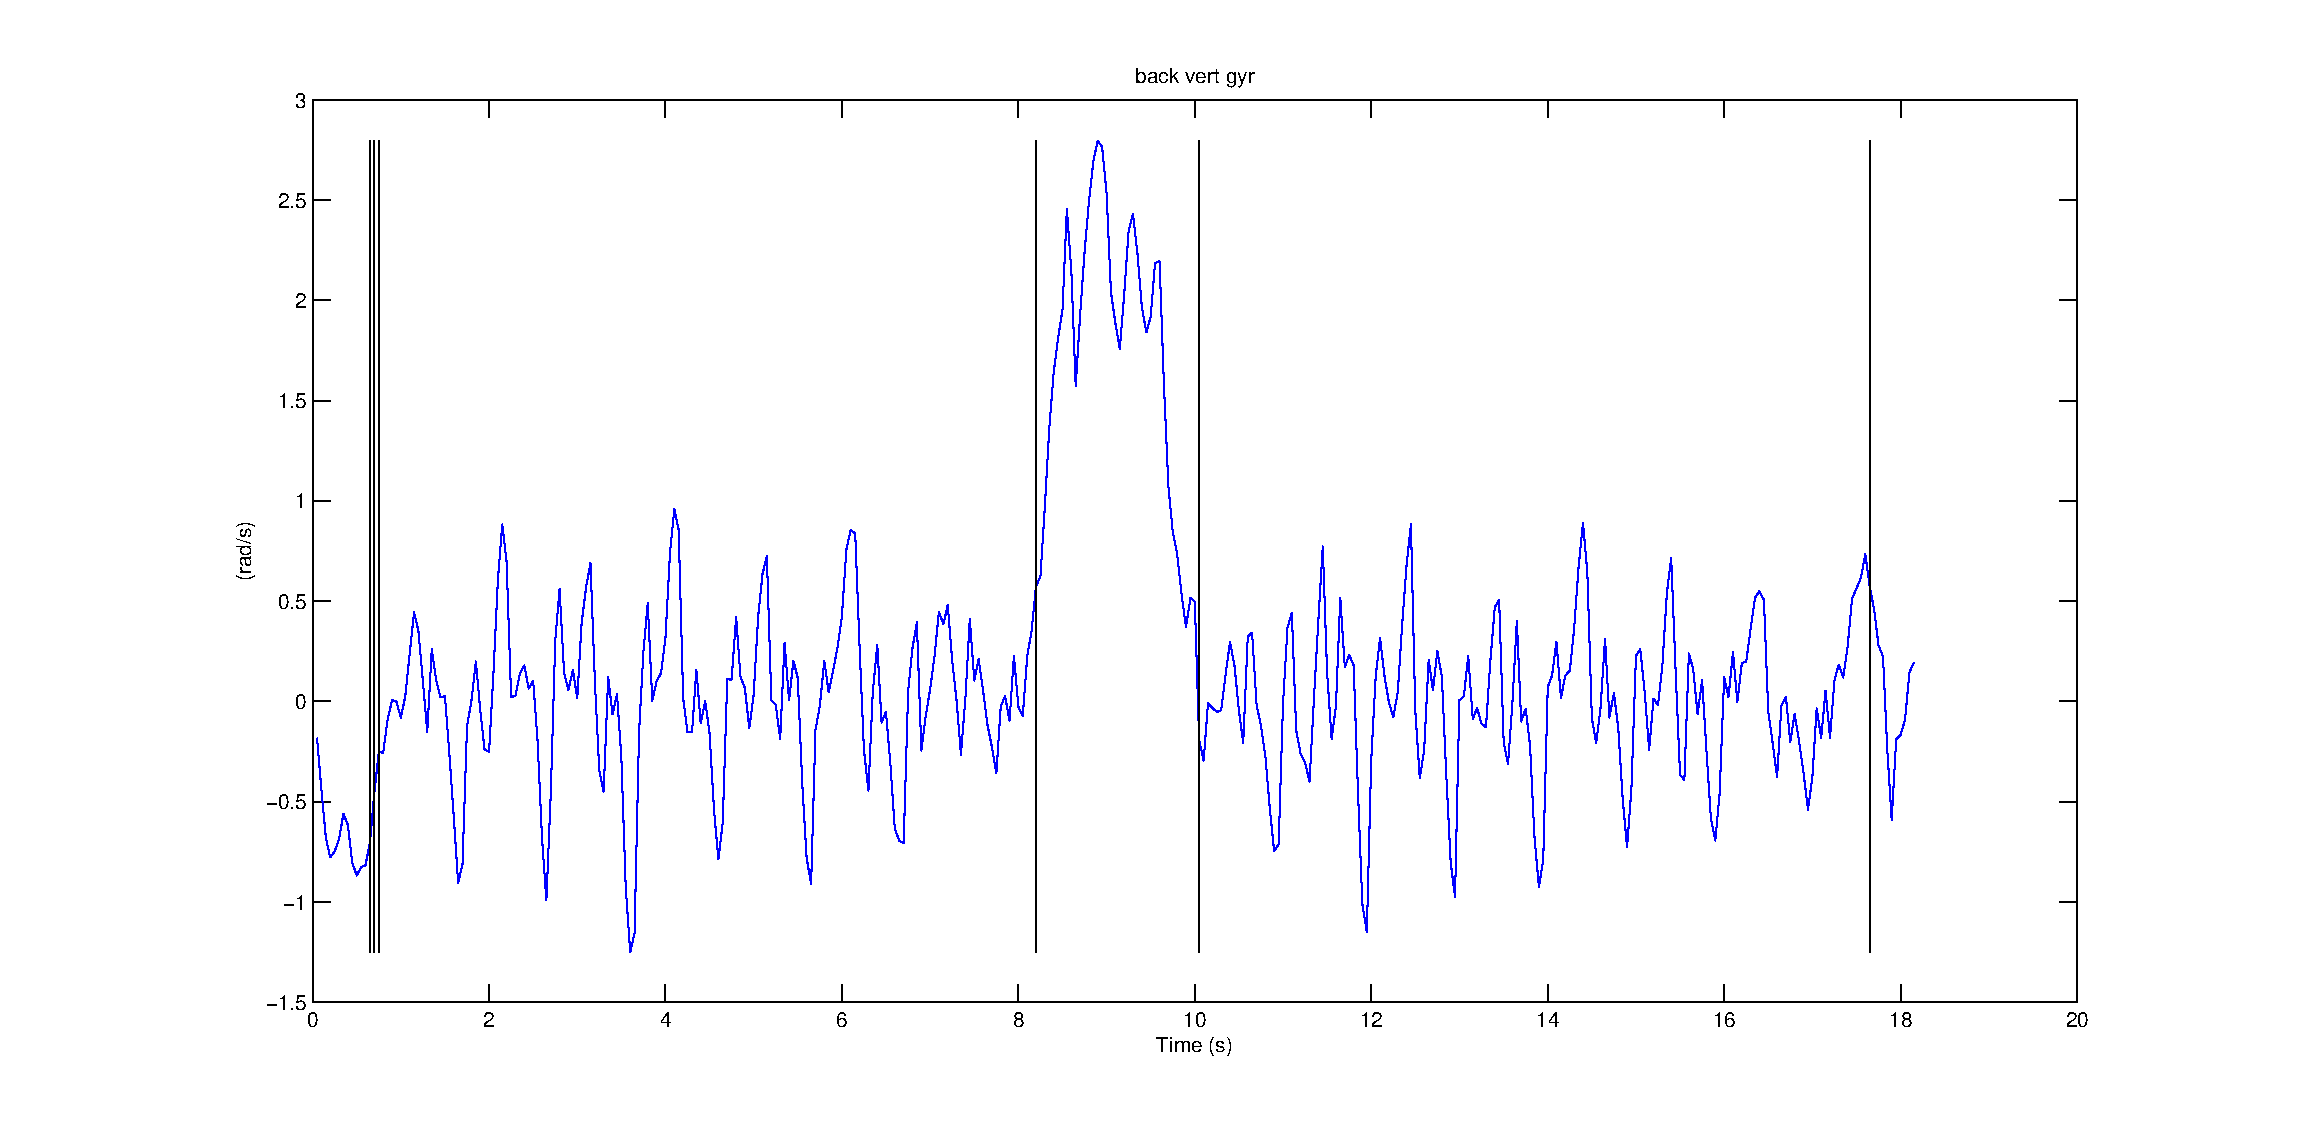
\includegraphics[scale=0.4]{examplecusumbackvertgyr}
\end{frame}

\end{document}